%! TEX program = xelatex
\documentclass[xetex]{beamer}

\usepackage{tikz}
\usetikzlibrary{shapes.geometric}
\usepackage{caption}
\usepackage{subfig}
\usepackage{graphicx}
\usepackage{hyperref}
\usepackage{siunitx}

\DeclareGraphicsExtensions{.pdf,.png,.jpg}

\usetheme[
	titleformat=smallcaps,
	sectionpage=progressbar,
	numbering=fraction,
]{metropolis}

% Tikz Commands
\newcommand{\rectnode}[3]{rectangle +(#1,#2) node[pos=0.5,font=\tiny] {#3}}
\newcommand{\squarenode}[2]{\rectnode{#1}{#1}{#2}}

\title{Pengembangan Keandalan Sistem ARINC 653\\dengan Menggunakan\\ \textit{Fault Tolerant Partition Scheduling}}
\subtitle{Sidang Tugas Akhir}
\author{Aufar Gilbran - 13513015}
\date{8 Agustus 2017}

\hypersetup{pdfstartview={FitH}}

\begin{document}
\frame{\titlepage}
\begin{frame}{Alur}
	\tableofcontents
\end{frame}

\section{Latar Belakang}
\begin{frame}
	\frametitle{Latar Belakang --- Definisi Sistem \textit{Real-Time}}
	\begin{itemize}
		\item Menurut Kang G. Shin, berikut merupakan komponen dari sebuah sistem \textit{real-time}: 
			\begin{itemize}
				\item \textit{Task} pada sistem memiliki \textit{deadline}.
				\item Keandalan sistem sangat penting.
			\end{itemize}
	\end{itemize}
\end{frame}
\begin{frame}
	\frametitle{Latar Belakang --- Sistem \textit{Real-Time} pada Avionika}
	\begin{itemize}
		\item Sistem \textit{real-time} digunakan pada berbagai bidang.
		\item Fokus penelitian adalah pada bidang avionika.
		\item Kegagalan sistem pada bidang avionika dapat mengakibatkan hilangnya nyawa atau kerusakan lingkungan.
		\item Contoh sistem \textit{real-time} pada bidang avionika:
			\begin{itemize}
				\item \textit{Aircraft Collision Avoidance System}.
				\item \textit{Aircraft Flight Control System}.
				\item \textit{Missile Approach Warning System}.
			\end{itemize}
	\end{itemize}
\end{frame}
\begin{frame}
	\frametitle{Latar Belakang --- ARINC 653}
	\begin{itemize}
		\item Standar untuk sistem operasi \textit{real-time} pada avionik.
		\item Menjamin lingkungan eksekusi layanan terpartisi pada sistem operasi ARINC 653.
		\item Sistem terpartisi mengakibatkan kegagalan yang terjadi pada suatu partisi terisolasi dan tidak mempengaruhi partisi lain.
		\item Kegagalan pada partisi tetap terjadi sehingga memungkinkan terjadinya kegagalan pada sistem secara keseluruhan.
	\end{itemize}
\end{frame}
\begin{frame}{Latar Belakang --- ARINC 653 \textit{Scheduler}}
	\begin{itemize}
		\item Isolasi waktu CPU pada sistem ARINC 653 dilakukan dengan menggunakan dua jenis \textit{scheduler}:
			\begin{itemize}
				\item \textit{Partition Scheduler} --- Menjadwalkan partisi-partisi pada sistem.
				\item \textit{Process Scheduler} --- Menjadwalkan layanan pada masing-masing partisi.
			\end{itemize}
		\item Fokus penelitian adalah \textit{partition scheduler}.
	\end{itemize}
\end{frame}
\begin{frame}
	\frametitle{Latar Belakang --- Xen}
	\begin{itemize}
		\item Xen merupakan solusi \textit{virtual machine} yang gratis dan \textit{open source}.
		\item Setiap \textit{virtual machine} pada Xen memiliki lingkungan eksekusi yang
			terisolasi sehingga dapat digunakan untuk memodelkan partisi pada
			spesifikasi ARINC 653. 
		\item \textit{Open source} $\implies$ Mudah melakukan modifikasi pada sistem:
		\item Teknologi lain yang serupa:
			\begin{itemize}
				\item VMWare ESXi
				\item Microsoft Hyper-V
				\item Oracle VM Server
			\end{itemize}
	\end{itemize}
\end{frame}
\begin{frame}
	\frametitle{Latar Belakang --- ARLX}
	\begin{itemize}
		\item Prototipe sistem yang memenuhi standar ARINC 653.
		\item Dikembangkan diatas Xen  $\implies$ memiliki karakteristik dan keuntungan Xen.
	\end{itemize}
\end{frame}
\begin{frame}
	\frametitle{Latar Belakang --- \textit{Fault-Tolerant Partition Scheduling}}
	\begin{itemize}
		\item Algoritma \textit{scheduling} partisi yang menggunakan partisi cadangan untuk menggantikan partisi asli apabila mengalami kegagalan.
		\item Solusi untuk meningkatkan keandalan sistem terpartisi.
		\item Cocok digunakan untuk sistem ARINC 653.
		\item Teknologi yang menggunakannya merupakan produk komersial.
	\end{itemize}
\end{frame}

\section{Rumusan Masalah \& Tujuan}
\begin{frame}
	\frametitle{Rumusan Masalah}
	\begin{itemize}
		\item Standar ARINC 653 tidak membuat sistem menjadi andal.
		\item Sistem ARINC 653 yang andal belum tersedia secara gratis dan \textit{open source}.
	\end{itemize}
\end{frame}
\begin{frame}
	\frametitle{Tujuan}
	\begin{itemize}
		\item Meningkatkan keandalan sistem ARINC 653.
		\item Dapat dicapai dengan:
			\begin{itemize}
				\item Implementasi \textit{fault-tolerant partition scheduling} pada sistem ARINC 653.
				\item Pengujian \textit{fault-tolerant partition scheduler} pada sistem ARINC 653.
				\item Analisis efektivitas \textit{fault-tolerant partition scheduling} pada sistem ARINC 653.
				\item Analisis efisiensi \textit{fault-tolerant partition scheduling} pada sistem ARINC 653.
			\end{itemize}
	\end{itemize}.
\end{frame}
\begin{frame}
	\frametitle{Batasan Masalah}
	\begin{itemize}
		\item Implementasi hanya akan dilakukan pada sistem dengan arsitektur x86-64.
		\item Implementasi hanya akan dilakukan di atas \textit{virtual machine}.
		\item Implementasi hanya akan diuji coba dengan menggunakan sistem operasi Linux untuk setiap partisi-nya.
			Hasil pada sistem operasi lain mungkin berbeda.
	\end{itemize}
\end{frame}

\section{Rancangan Solusi dan Pengujian}
\begin{frame}
	\frametitle{Rancangan Solusi --- ARLX}
	\begin{itemize}
		\item Memodelkan partisi dengan menggunakan \textit{virtual machine}.
		\item Menggunakan \textit{major time frame} (didapat dari faktor persekutuan
			terbesar \textit{deadline} seluruh partisi).
		\item Partisi akan meminta \textit{slot} pada \textit{major time frame}.
	\end{itemize}
\end{frame}
\begin{frame}
	\frametitle{Rancangan Solusi --- Daftar Jadwal}
	\begin{itemize}
		\item Modifikasi jadwal pada ARLX.
		\item Setiap \textit{entry} merupakan sebuah layanan.
		\item Masing-masing \textit{entry}/layanan memiliki daftar partisi penyedia.
	\end{itemize}
	\centering
	\begin{figure}
		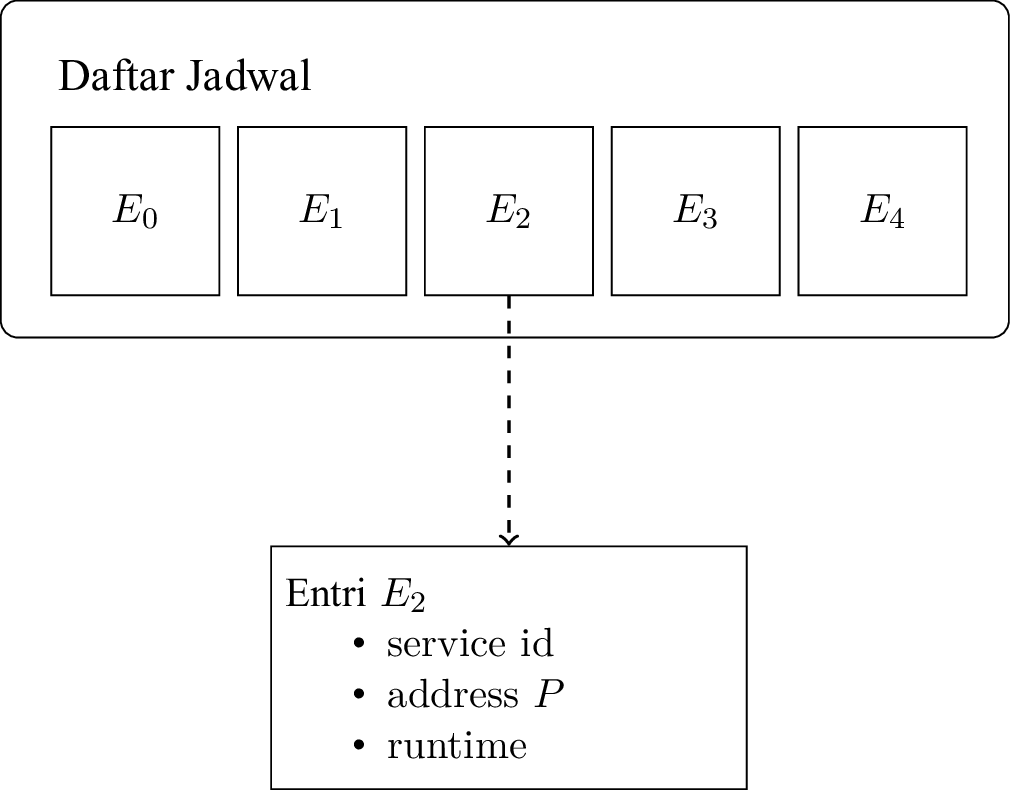
\includegraphics[scale=0.15]{./final-project-figure0.png}
		\caption{Daftar Jadwal}
	\end{figure}
\end{frame}
\begin{frame}
	\frametitle{Rancangan Solusi --- Algoritma \textit{Scheduling}}
	\begin{itemize}
		\item Secara umum sama dengan algoritma \textit{partition scheduling} pada ARINC 653.
		\item Asumsikan setiap partisi menyediakan layanan.
		\item Partisi \textit{backup} memiliki layanan yang sama dengan partisi \textit{primary}.
		\item \textit{Scheduler} hanya akan memberikan CPU kepada
			partisi yang tidak sedang mengalami kegagalan
			dan layanan tersebut belum pernah tersedia.
		\item Layanan belum pernah disediakan
			$\Longleftrightarrow$ tidak ada partisi dengan layanan
			tersebut yang sudah diberikan waktu CPU pada suatu
			\textit{major time frame}.
	\end{itemize}
\end{frame}
\begin{frame}
	\frametitle{Rancangan Solusi --- Informasi Partisi}
	\begin{itemize}
		\item \textit{Scheduler} perlu mengetahui informasi terkait status partisi pada partisi.
		\item Status partisi diperlukan untuk mengetahui apakah partisi mengalami kegagalan/tidak.
		\item Informasi tersebut dapat diberikan oleh partisi melalui \textit{hypercall}.
	\end{itemize}
\end{frame}
\begin{frame}{Rancangan Solusi --- Alur Informasi Sistem}
	\centering
	\begin{figure}
		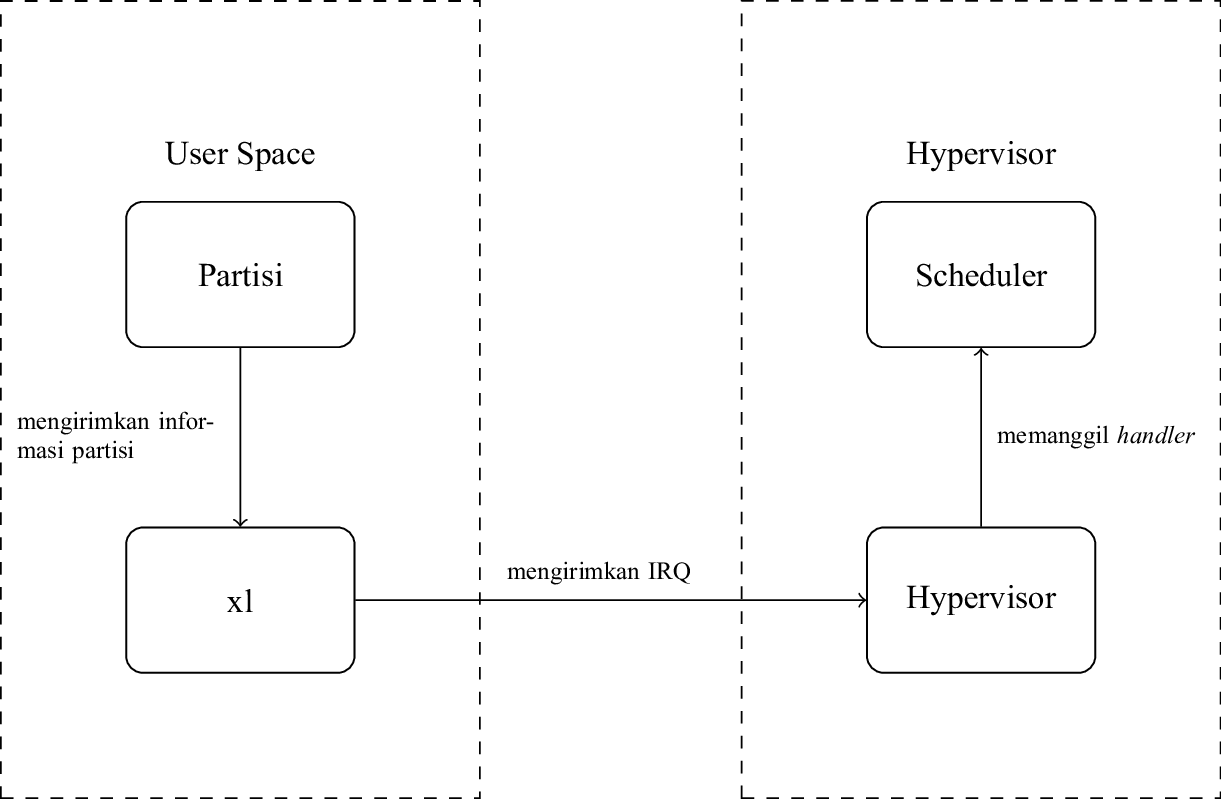
\includegraphics[scale=0.23]{./final-project-figure1.png}
		\caption{Alur informasi sistem}
	\end{figure}
\end{frame}
\begin{frame}{Rancangan Solusi --- Flowchart Algoritma \textit{Scheduling}}
	\centering
	\begin{figure}
		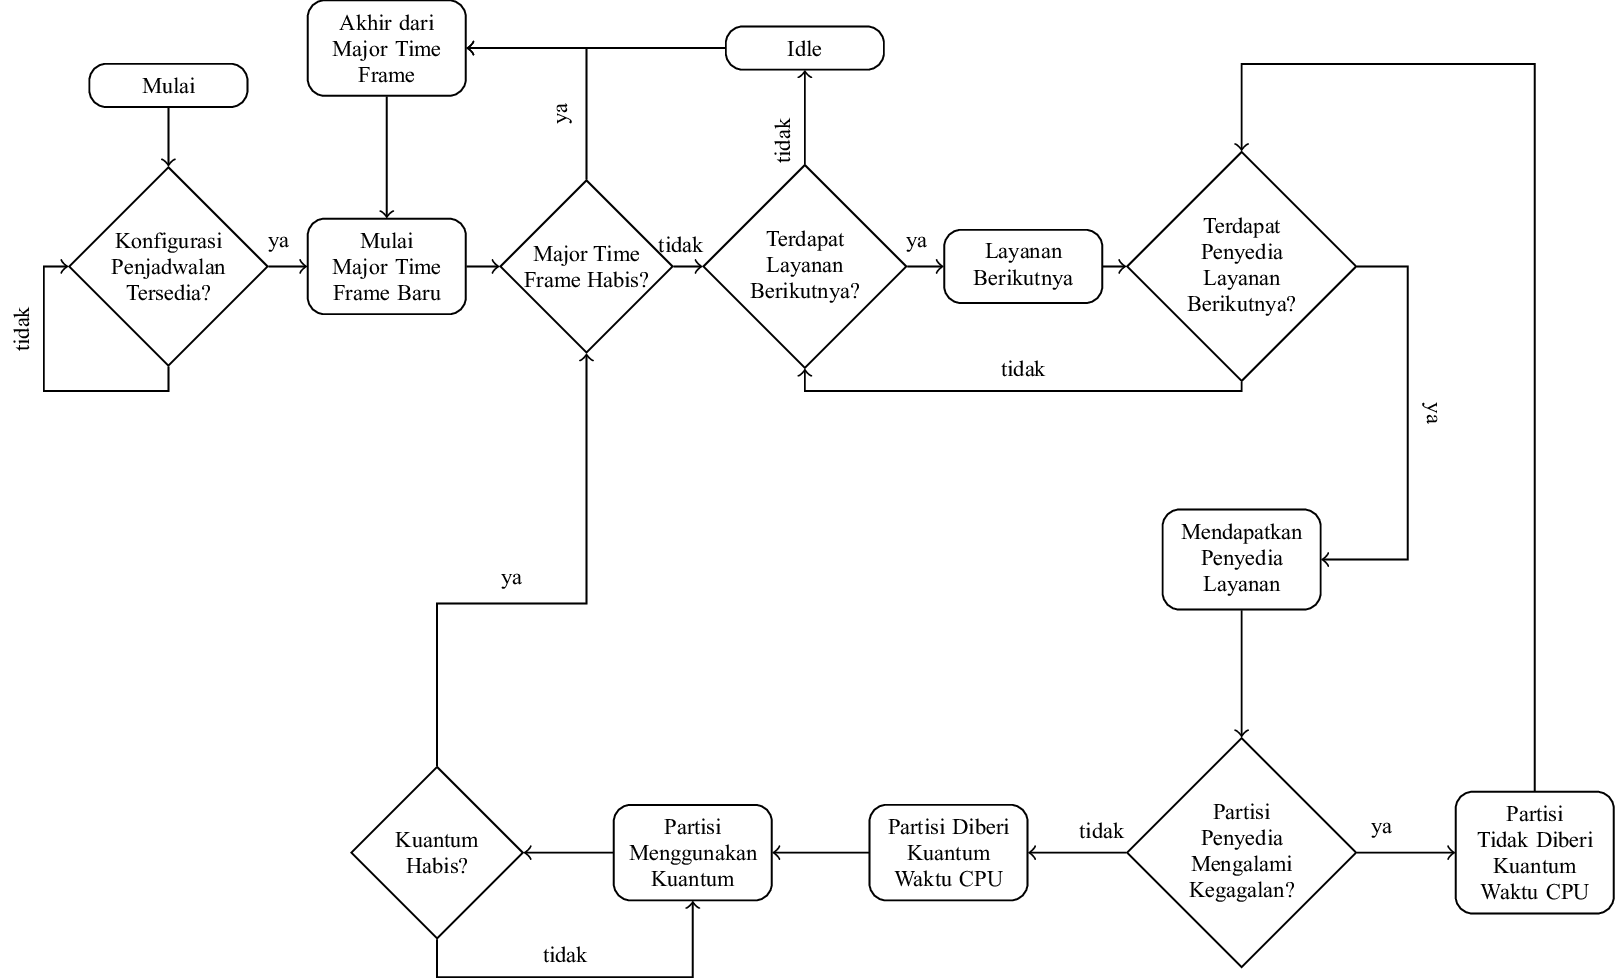
\includegraphics[scale=0.18]{./final-project-figure2.png}
		\caption{Diagram \textit{Flowchart} Algoritma \textit{Scheduling}}
	\end{figure}
\end{frame}
\begin{frame}{Rancangan Solusi --- Ilustrasi Algoritma}
	\centering
	\begin{figure}
		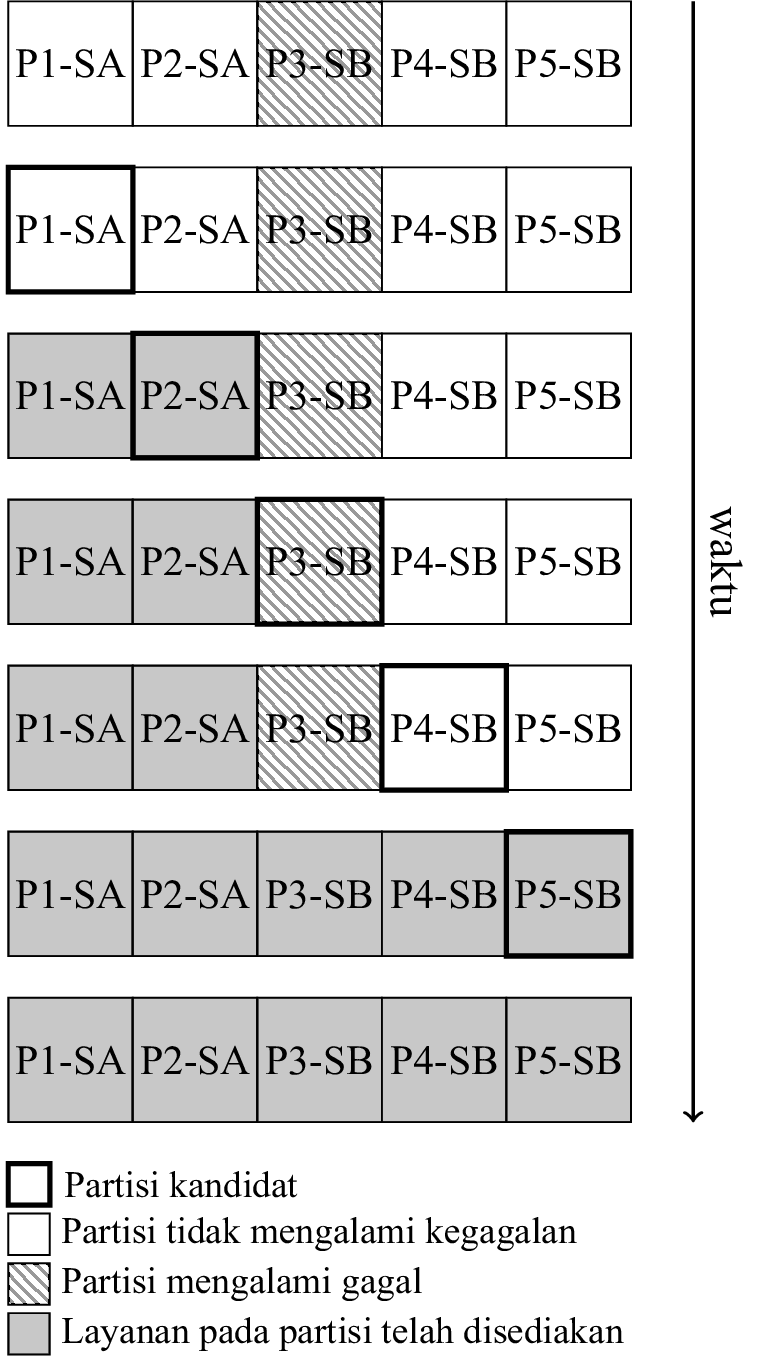
\includegraphics[scale=0.15]{./final-project-figure3.png}
		\caption{Contoh \textit{primary-backup scheduling}}
	\end{figure}
\end{frame}
\begin{frame}{Rancangan Pengujian -- Pengujian Keandalan}
	\begin{itemize}
		\item Metode:
			\begin{enumerate}
				\item Partisi akan diuji dengan arsitektur \textit{client-server}.
				\item Partisi sebagai \textit{client} mengirimkan \textit{heartbeat} ke \textit{server}.
				\item \textit{Server} mencatat nomor identifikasi partisi.
			\end{enumerate}
		\item Tujuan:
			\begin{enumerate}
				\item Mengetahui jumlah layanan yang disediakan pada setiap \textit{major time frame}.
				\item Menjamin partisi yang diberi waktu CPU adalah partisi yang seharusnya.
				\item Menghitung \textit{latency} layanan
			\end{enumerate}
	\end{itemize}
\end{frame}
\begin{frame}{Rancangan Pengujian -- Pengujian \textit{Latency}}
	\begin{itemize}
		\item Metode:
			\begin{enumerate}
				\item Partisi akan menjalankan \textit{periodic task}.
				\item \textit{Periodic task} akan mengukur \textit{latency}.
				\item Hasil pengukuran seluruhnya akan dicatat pada \textit{file}.
			\end{enumerate}
		\item Tujuan:
			\begin{enumerate}
				\item Menghitung \textit{latency} \textit{periodic task}
				\item Menjamin \textit{task} akan dijalankan sebelum \textit{deadline}.
				\item Menjamin tidak terjadi \textit{time-drift} yang signifikan.
			\end{enumerate}
	\end{itemize}
\end{frame}
\begin{frame}{Rancangan Pengujian -- Arsitektur Kerangka Uji}
	\centering
	\begin{figure}
		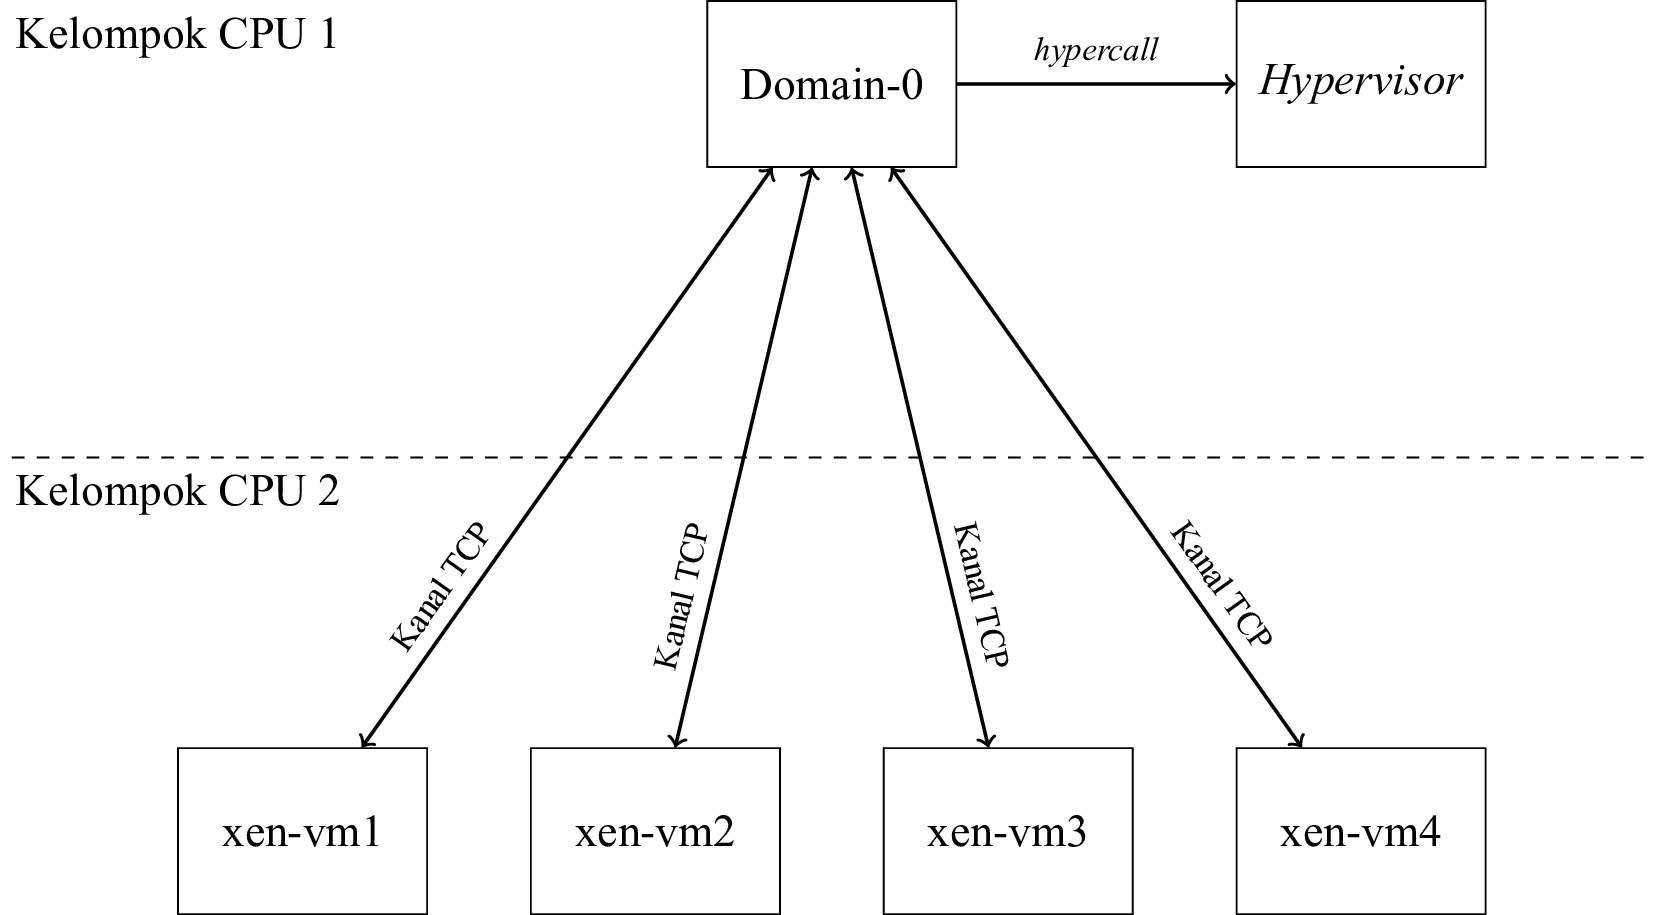
\includegraphics[scale=0.20]{./final-project-figure4.png}
		\caption{Arsitektur Kerangka Uji}
	\end{figure}
\end{frame}
\begin{frame}{Rancangan Pengujian -- Cara Kerja Kerangka Uji}
	\centering
	\begin{figure}
		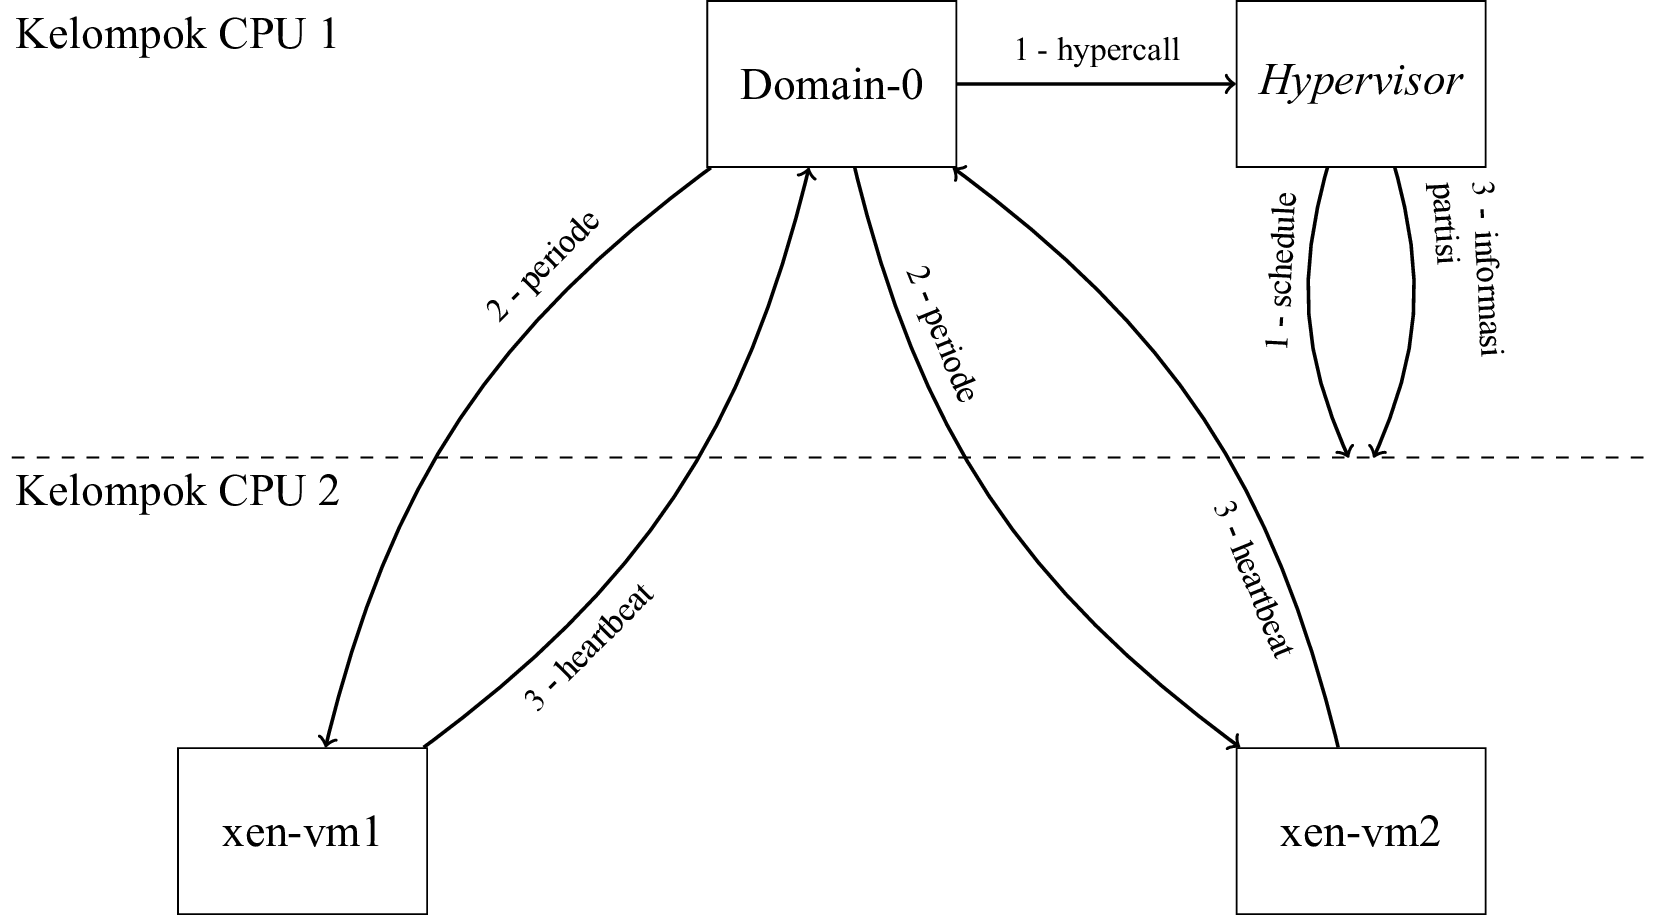
\includegraphics[scale=0.20]{./final-project-figure5.png}
		\caption{Cara Kerja Kerangka Uji}
	\end{figure}
\end{frame}

\section{Implementasi}
\begin{frame}
	\frametitle{Implementasi --- \textit{Hypercall}}
	\begin{itemize}
		\item Partisi dapat mengirimkan informasi partisi kepada \textit{scheduler}.
		\item Menggunakan \textit{interface} pada Xen untuk mendefinisikan \textit{public hypercall}.
		\item Menggunakan libxl pada Xen untuk membuat kakas pada \textit{user space}.
	\end{itemize}
\end{frame}
\begin{frame}
	\frametitle{Implementasi --- \textit{Primary-Backup Partition Scheduling}}
	\begin{itemize}
		\item \textit{Scheduler} dapat menyimpan informasi partisi.
		\item \textit{Scheduler} dapat menentukan pemberian waktu CPU kepada partisi berdasarkan keadaan dan layanan pada partisi tersebut.
		\item \textit{Scheduler} dapat menjamin penjadwalan yang deterministik.
		\item Menggunakan \textit{interface} pada Xen untuk mendefinisikan \textit{scheduler}.
	\end{itemize}
\end{frame}
\section{Pengujian}

\begin{frame}{Pengujian -- Parameter Pengujian}
	\begin{itemize}
		\item Delta \textit{Timing}, untuk melihat perbandingan \textit{timing} dengan periode ekspektasi.

			\begin{equation*}
				delta = now - last
			\end{equation*}

		\item Galat \textit{Timing}, untuk melihat selisih \textit{timing} dengan periode ekspektasi.

			\begin{equation*}
				galat = delta - expected
			\end{equation*}


	\end{itemize}
\end{frame}

\begin{frame}{Pengujian -- Keandalan (Skenario 1)}
	\begin{itemize}
		\item Jumlah layanan = 1 @ \SI{20}{\milli\second}.
		\item Jumlah partisi penyedia = 1.
		\item \textit{Major time frame} = \SI{20}{\milli\second}.
	\end{itemize}
\end{frame}

\begin{frame}{Pengujian -- Keandalan (Skenario 1)}
	\begin{figure}[htbp]
		\centering
		\begin{tabular}{c}
			\subfloat{
				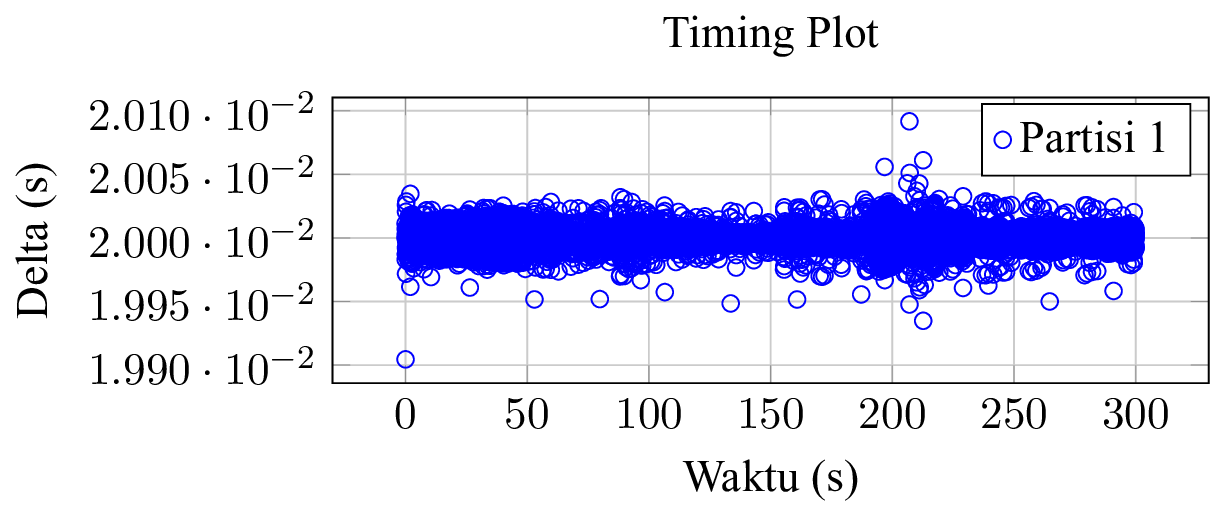
\includegraphics[scale=0.15]{./reliability-s1-delta.png}
			} \\
			\subfloat{
				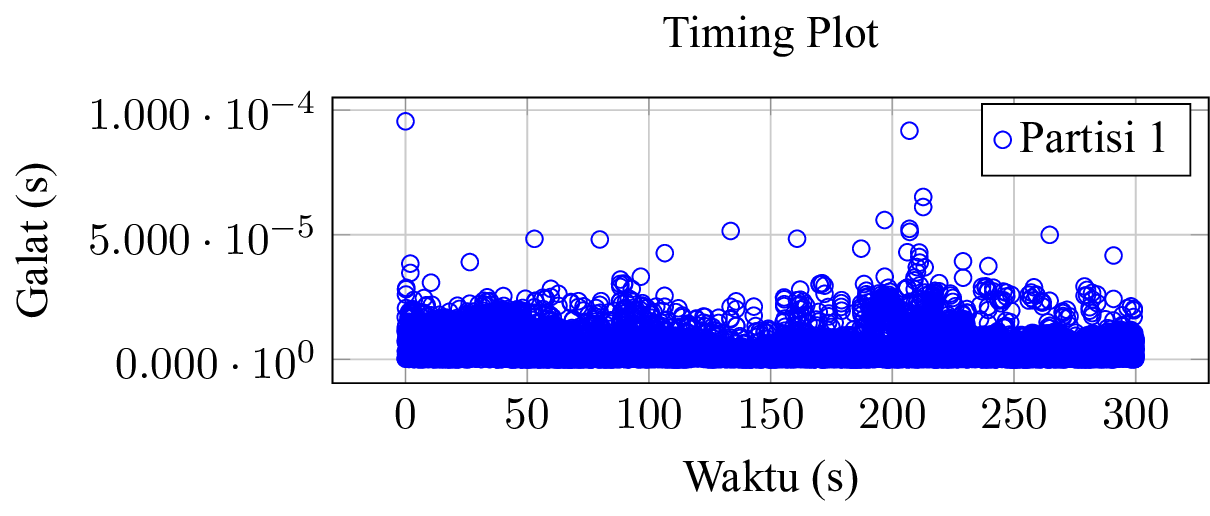
\includegraphics[scale=0.15]{./reliability-s1-error.png}
			}
		\end{tabular}
		\caption{Hasil pengujian keandalan skenario 1}
	\end{figure}
\end{frame}

\begin{frame}{Pengujian -- Keandalan (Skenario 2)}
	\begin{itemize}
		\item Jumlah layanan = 1 @ \SI{20}{\milli\second}.
		\item Jumlah partisi penyedia = 2.
		\item \textit{Major time frame} = \SI{20}{\milli\second}.
	\end{itemize}
\end{frame}
\begin{frame}{Pengujian -- Keandalan (Skenario 2)}
	\begin{figure}[htbp]
		\centering
		\begin{tabular}{c}
			\subfloat{
				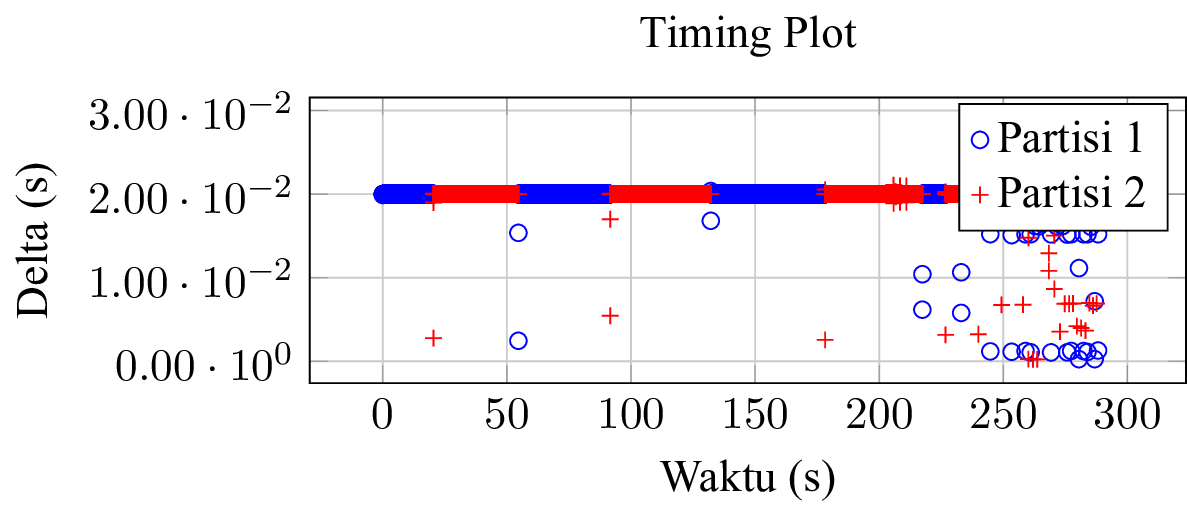
\includegraphics[scale=0.15]{./reliability-s2-delta.png}
			} \\
			\subfloat{
				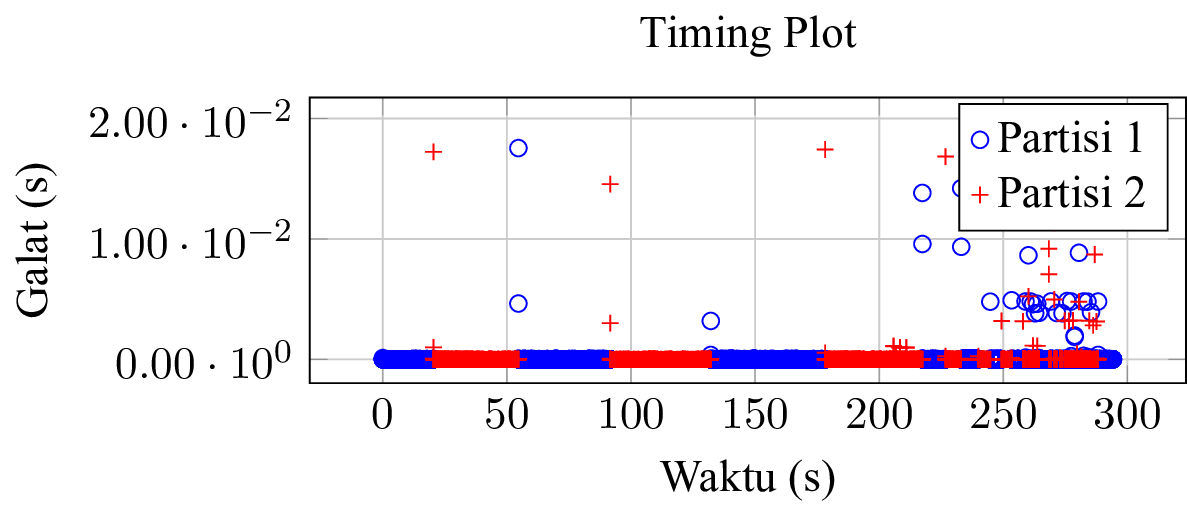
\includegraphics[scale=0.15]{./reliability-s2-error.png}
			}
		\end{tabular}
		\caption{Hasil pengujian keandalan skenario 2}
	\end{figure}
\end{frame}

\begin{frame}{Pengujian -- Keandalan (Skenario 3)}
	\begin{itemize}
		\item Jumlah layanan = 9 @ \SI{20}{\milli\second}.
		\item Jumlah partisi penyedia = 1.
		\item \textit{Major time frame} = \SI{180}{\milli\second}.
	\end{itemize}
\end{frame}
\begin{frame}{Pengujian -- Keandalan (Skenario 3)}
	\begin{figure}[htbp]
		\centering
		\begin{tabular}{c}
			\subfloat{
				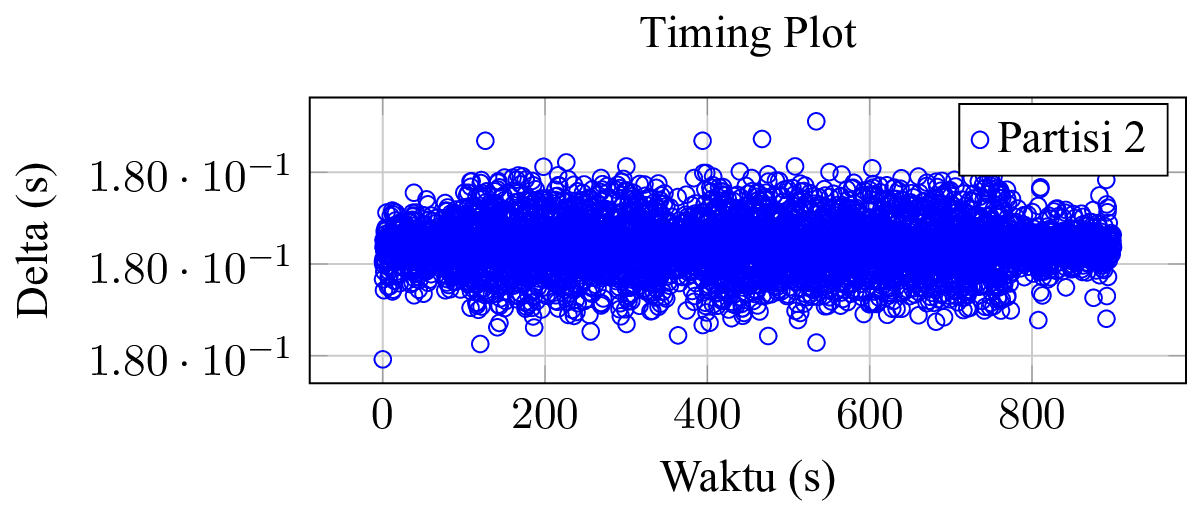
\includegraphics[scale=0.15]{./reliability-s3-delta-p2.png}
			} \\
			\subfloat{
				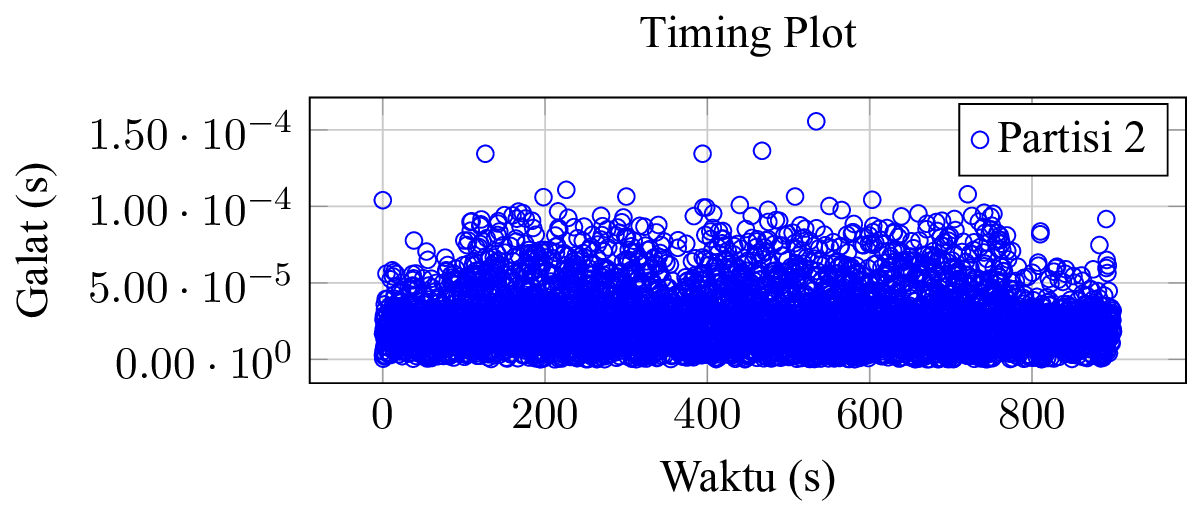
\includegraphics[scale=0.15]{./reliability-s3-error-p2.png}
			}
		\end{tabular}
		\caption{Hasil pengujian keandalan skenario 3 (hasil baik)}
	\end{figure}
\end{frame}
\begin{frame}{Pengujian -- Keandalan (Skenario 3)}
	\begin{figure}[htbp]
		\centering
		\begin{tabular}{c}
			\subfloat{
				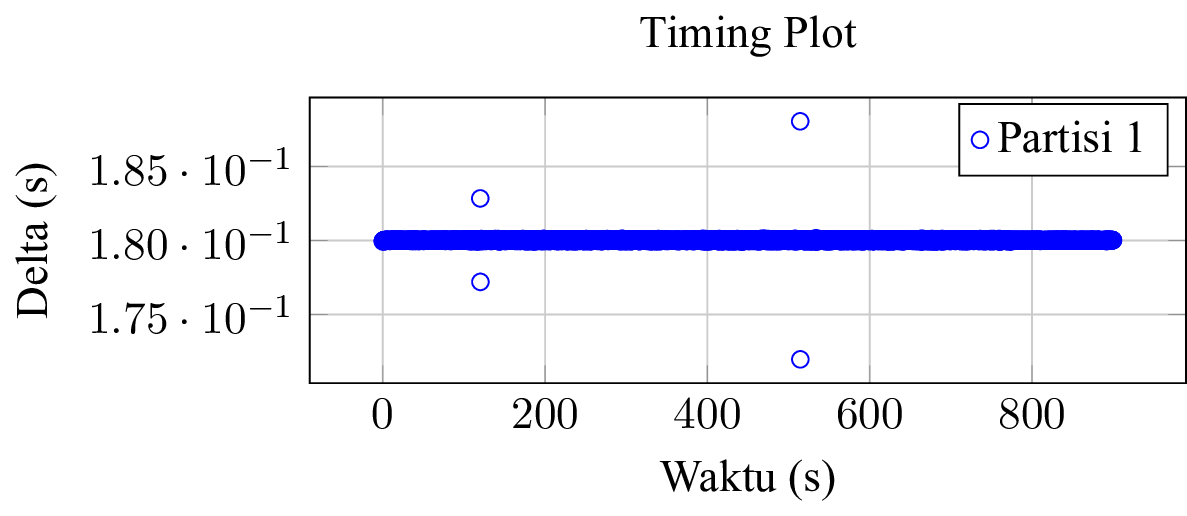
\includegraphics[scale=0.15]{./reliability-s3-delta-p1.png}
			} \\
			\subfloat{
				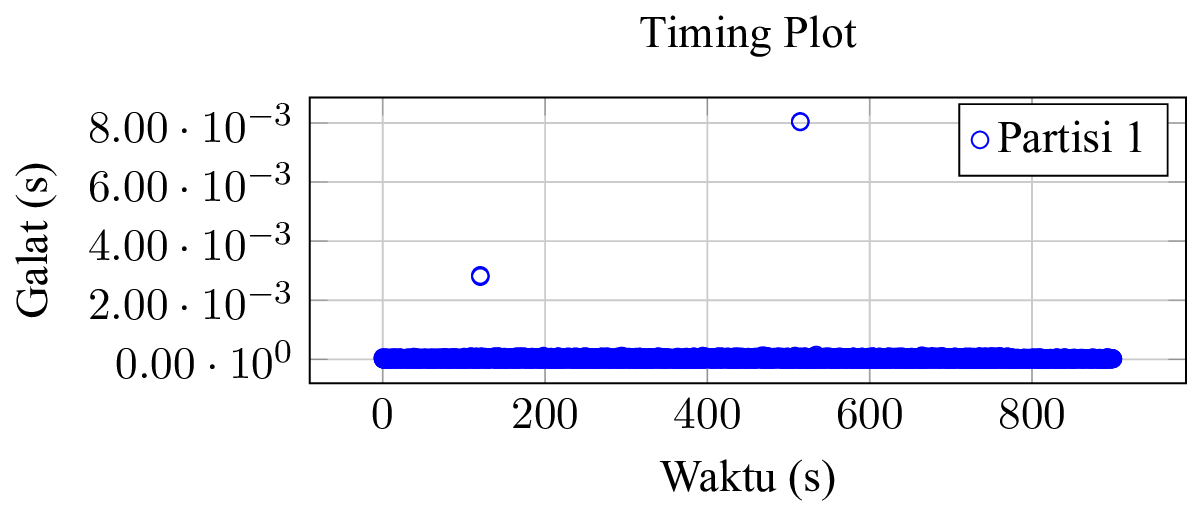
\includegraphics[scale=0.15]{./reliability-s3-error-1.png}
			}
		\end{tabular}
		\caption{Hasil pengujian keandalan skenario 3 (hasil buruk)}
	\end{figure}
\end{frame}


\begin{frame}{Pengujian -- Pengujian Keandalan (Skenario 4)}
	\begin{itemize}
		\item Jumlah layanan = 2 @ \SI{20}{\milli\second}.
		\item Jumlah partisi penyedia masing-masing layanan = 1.
		\item \textit{Major time frame} = \SI{180}{\milli\second}.
		\item Pada kasus ini, partisi penyedia merupakan partisi yang sama.
	\end{itemize}
\end{frame}
\begin{frame}{Pengujian -- Keandalan (Skenario 4)}
	\begin{figure}[htbp]
		\centering
		\begin{tabular}{c}
			\subfloat{
				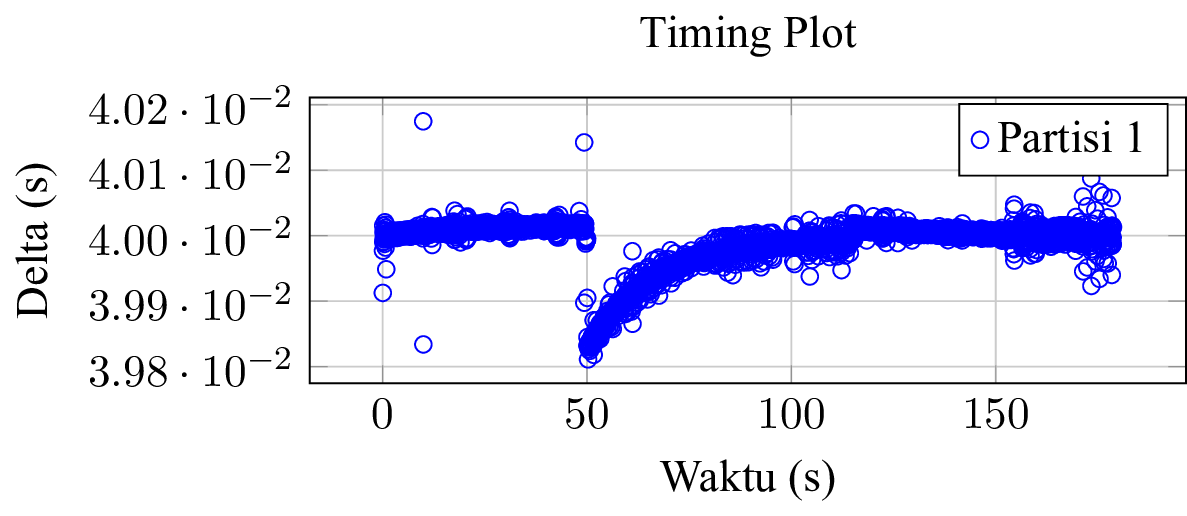
\includegraphics[scale=0.15]{./reliability-s4-delta.png}
			} \\
			\subfloat{
				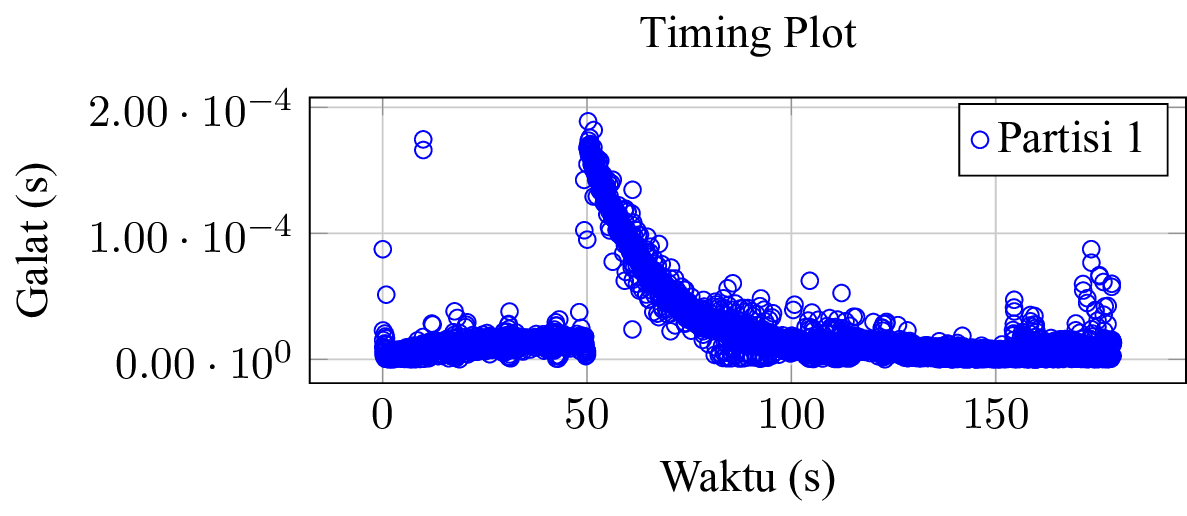
\includegraphics[scale=0.15]{./reliability-s4-error.png}
			}
		\end{tabular}
		\caption{Hasil pengujian keandalan skenario 4}
	\end{figure}
\end{frame}

\begin{frame}{Pengujian -- Pengujian Keandalan (Skenario 5)}
	\begin{itemize}
		\item Jumlah layanan = 4 @ \SI{10}{\milli\second}.
		\item Jumlah partisi penyedia masing-masing layanan = 2.
		\item Terdapat waktu \textit{idle} = \SI{10}{\milli\second}.
		\item \textit{Major time frame} = \SI{50}{\milli\second}.
	\end{itemize}
\end{frame}
\begin{frame}{Pengujian -- Keandalan (Skenario 5)}
	\begin{figure}[htbp]
		\centering
		\begin{tabular}{c}
			\subfloat{
				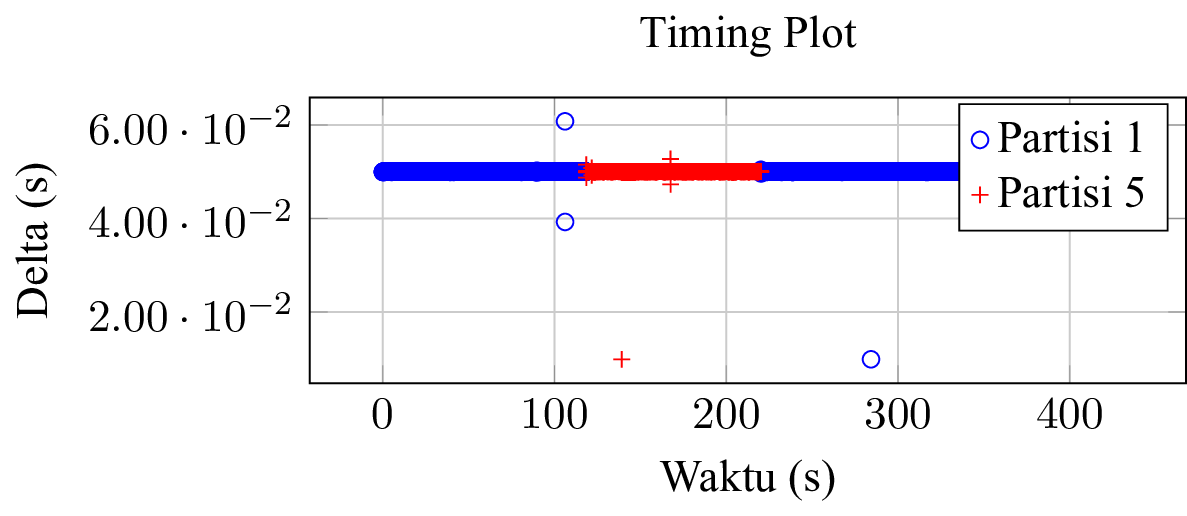
\includegraphics[scale=0.15]{./reliability-s5-delta-p1.png}
			} \\
			\subfloat{
				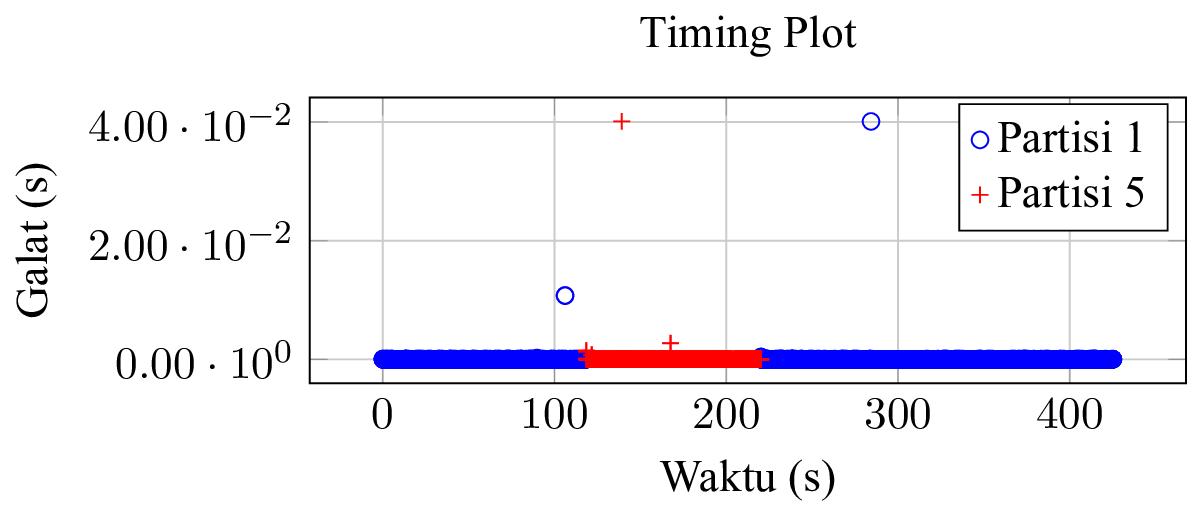
\includegraphics[scale=0.15]{./reliability-s5-error-p1.png}
			}
		\end{tabular}
		\caption{Hasil pengujian keandalan skenario 5}
	\end{figure}
\end{frame}

\begin{frame}{Pengujian -- Keandalan (Skenario 6)}
	\begin{itemize}
		\item Jumlah layanan = 3.
		\item Durasi layanan 1 = \SI{30}{\milli\second}.
		\item Durasi layanan 2 = \SI{20}{\milli\second}.
		\item Durasi layanan 3 = \SI{10}{\milli\second}.
		\item Jumlah partisi penyedia layanan 1 = 2.
		\item Jumlah partisi penyedia layanan 2 = 3.
		\item Jumlah partisi penyedia layanan 3 = 1.
		\item \textit{Major time frame} = \SI{60}{\milli\second}.
	\end{itemize}
\end{frame}
\begin{frame}{Pengujian -- Keandalan (Skenario 6)}
	\begin{figure}[htbp]
		\centering
		\begin{tabular}{c}
			\subfloat{
				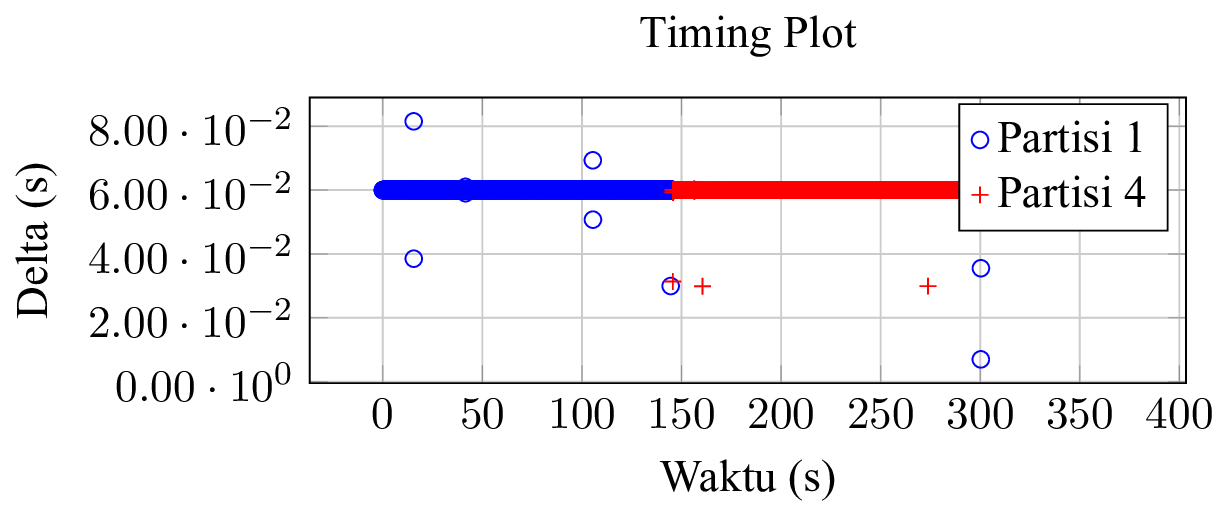
\includegraphics[scale=0.15]{./reliability-s6-delta-p1.png}
			} \\
			\subfloat{
				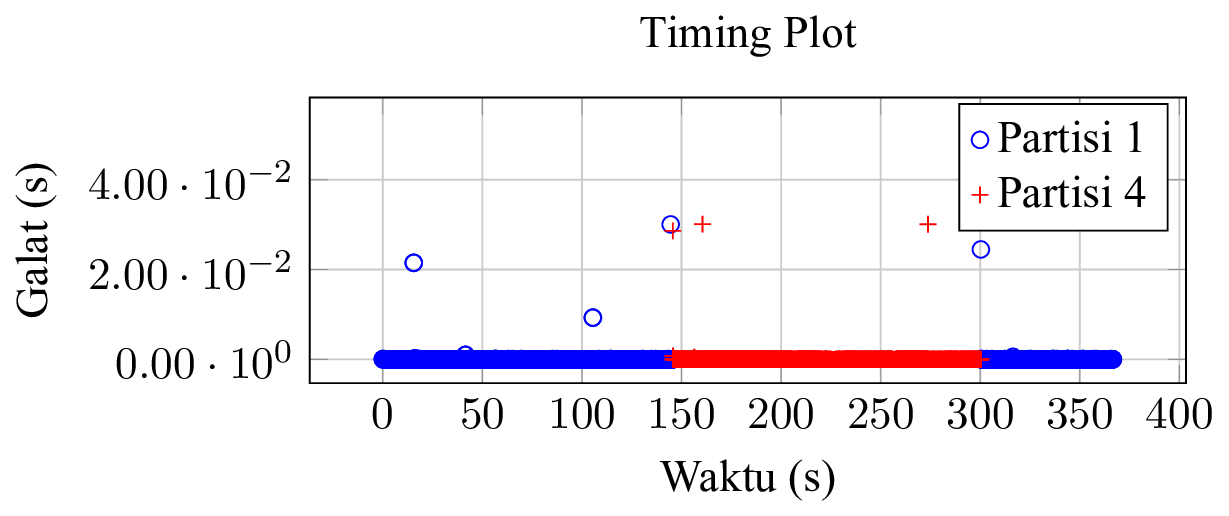
\includegraphics[scale=0.15]{./reliability-s6-error-p1.png}
			}
		\end{tabular}
		\caption{Hasil pengujian keandalan skenario 6 (layanan 1)}
	\end{figure}
\end{frame}
\begin{frame}{Pengujian -- Keandalan (Skenario 6)}
	\begin{figure}[htbp]
		\centering
		\begin{tabular}{c}
			\subfloat{
				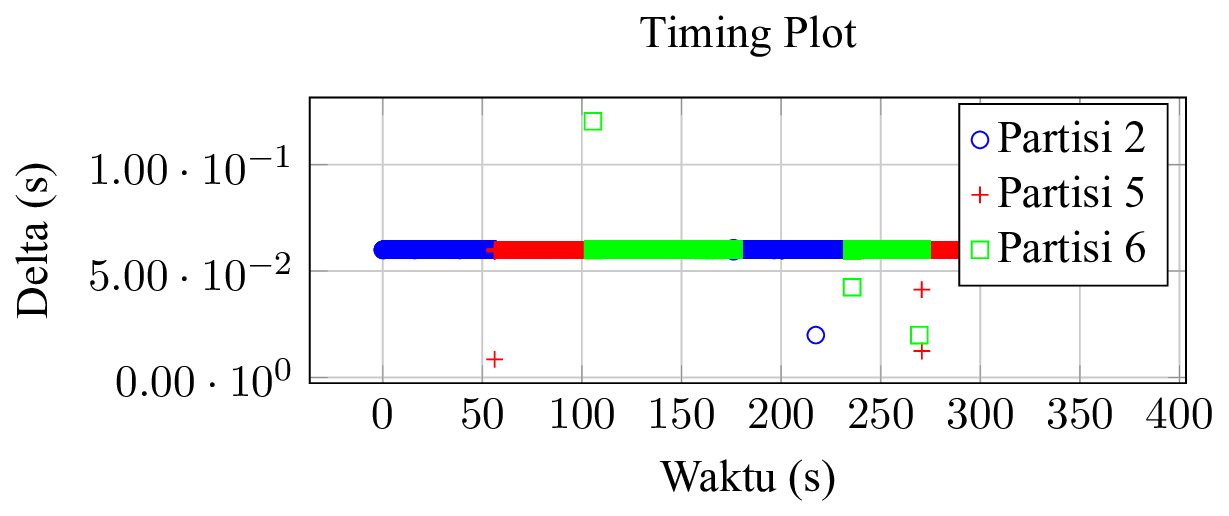
\includegraphics[scale=0.15]{./reliability-s6-delta-p2.png}
			} \\
			\subfloat{
				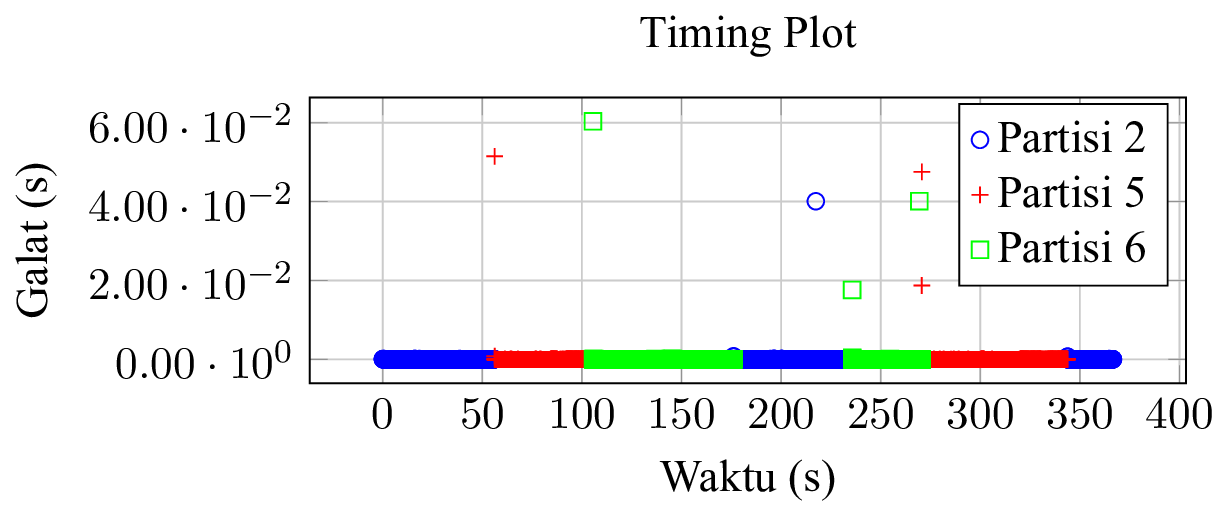
\includegraphics[scale=0.15]{./reliability-s6-error-p2.png}
			}
		\end{tabular}
		\caption{Hasil pengujian keandalan skenario 6 (layanan 2)}
	\end{figure}
\end{frame}
\begin{frame}{Pengujian -- Keandalan (Skenario 6)}
	\begin{figure}[htbp]
		\centering
		\begin{tabular}{c}
			\subfloat{
				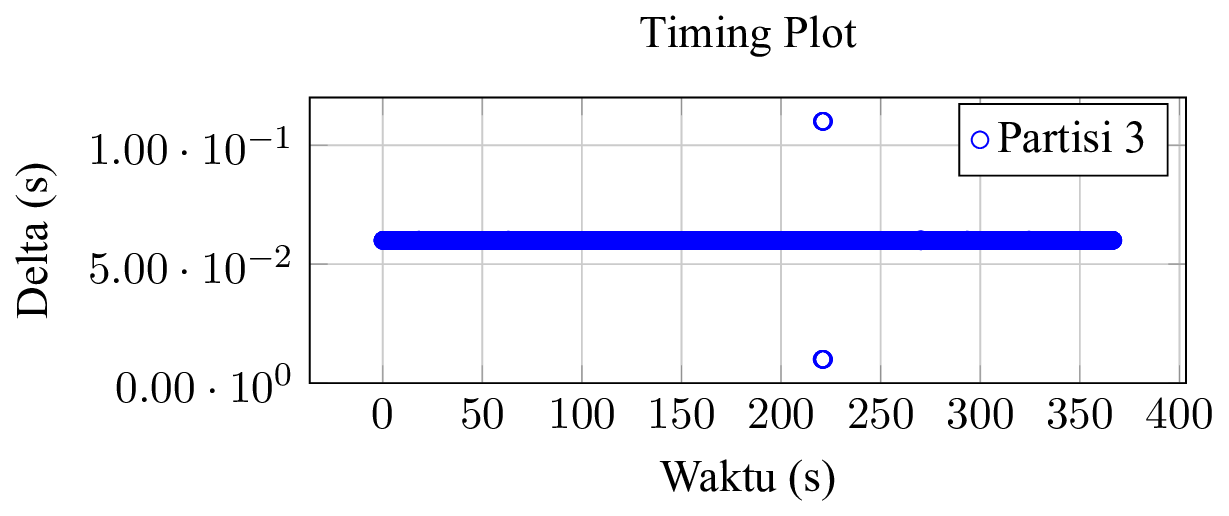
\includegraphics[scale=0.15]{./reliability-s6-delta-p3.png}
			} \\
			\subfloat{
				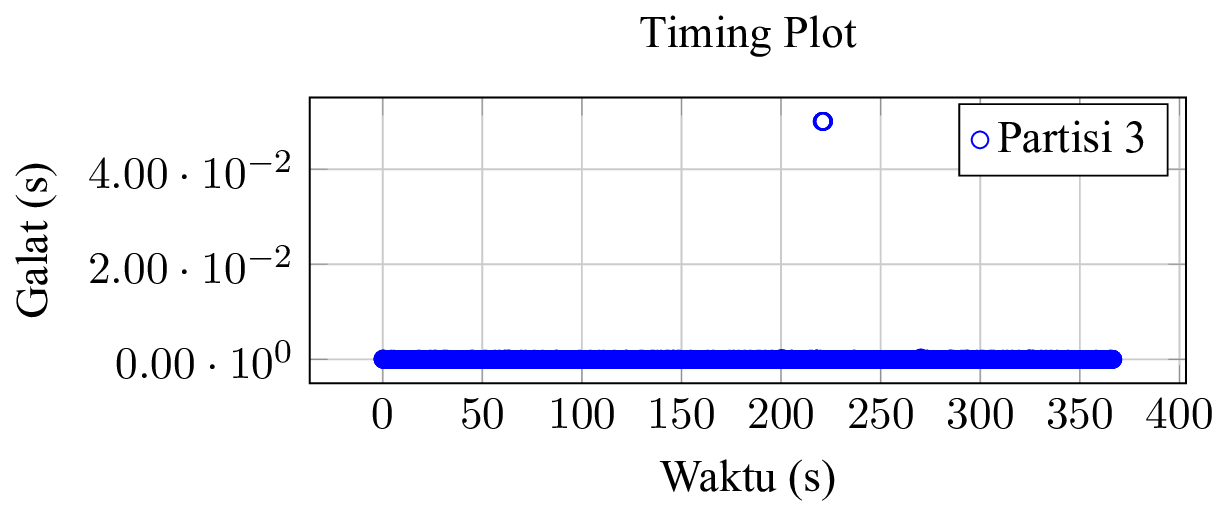
\includegraphics[scale=0.15]{./reliability-s6-error-p3.png}
			}
		\end{tabular}
		\caption{Hasil pengujian keandalan skenario 6 (layanan 3)}
	\end{figure}
\end{frame}

\begin{frame}{Pengujian -- Kesimpulan Pengujian Keandalan}
	\begin{enumerate}

		\item \textit{Scheduler} dapat melakukan penjadwalan partisi
			\textit{backup} ketika partisi \textit{primary}
			mengalami kegagalan.

		\item \textit{Scheduler} dapat melakukan penjadwalan partisi
			\textit{backup} dengan prioritas yang lebih rendah
			ketika partisi \textit{backup} yang memiliki prioritas
			lebih tinggi mengalami kegagalan.

		\item Apabila terdapat beberapa layanan, maka beberapa saat
			setelah pergantian partisi, terdapat \textit{latency}
			yang cukup tinggi.

	\end{enumerate}
\end{frame}

\begin{frame}{Pengujian -- Pengujian \textit{Latency} (Skenario 1)}
	\begin{itemize}
		\item Jumlah layanan = 1 @ \SI{20}{\milli\second}.
		\item \textit{Major time frame} = \SI{20}{\milli\second}.
	\end{itemize}
\end{frame}
\begin{frame}{Pengujian -- Pengujian \textit{Latency} (Skenario 1)}
	\begin{figure}[htbp]
		\centering
		\begin{tabular}{c}
			\subfloat{
				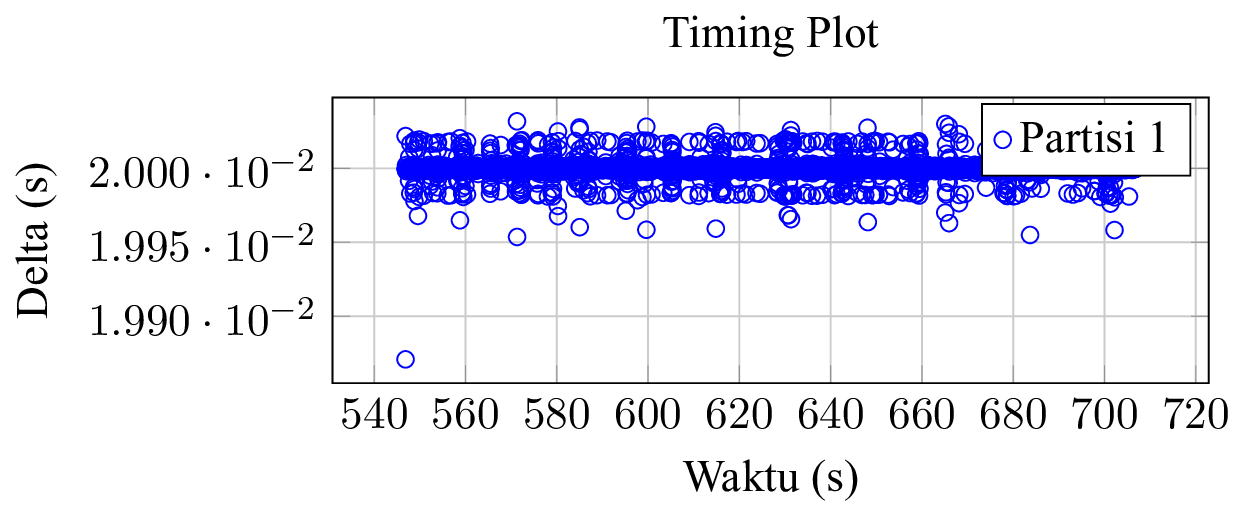
\includegraphics[scale=0.15]{./latency-s1-delta.png}
			} \\
			\subfloat{
				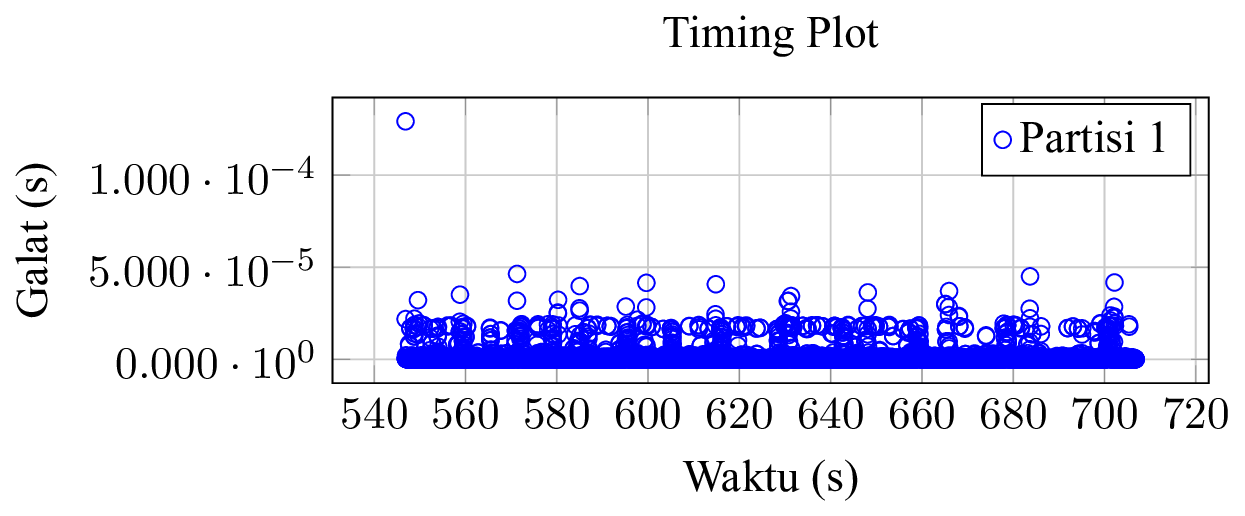
\includegraphics[scale=0.15]{./latency-s1-error.png}
			}
		\end{tabular}
		\caption{Hasil pengujian \textit{latency} (Skenario 1)}
	\end{figure}

\end{frame}

\begin{frame}{Pengujian -- Pengujian \textit{Latency} (Skenario 2)}
	\begin{itemize}
		\item Jumlah layanan = 4 @ \SI{10}{\milli\second}.
		\item Terdapat waktu \textit{idle} = \SI{10}{\milli\second}.
		\item \textit{Major time frame} = \SI{50}{\milli\second}.
	\end{itemize}
\end{frame}
\begin{frame}{Pengujian -- Pengujian \textit{Latency} (Skenario 2)}
	\begin{figure}[htbp]
		\centering
		\begin{tabular}{c}
			\subfloat{
				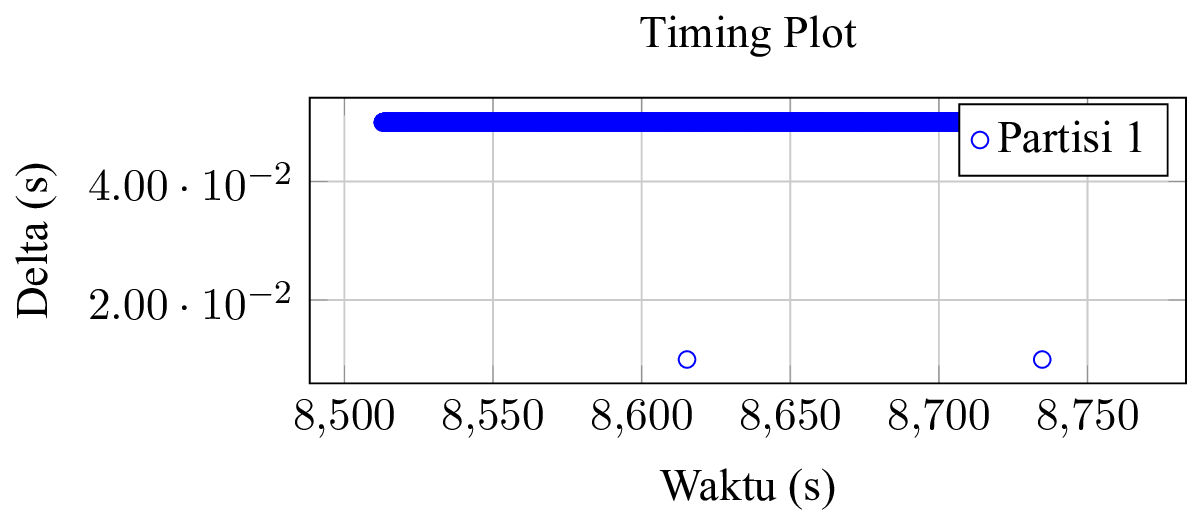
\includegraphics[scale=0.15]{latency-s2-delta-p1.png}
			} \\
			\subfloat{
				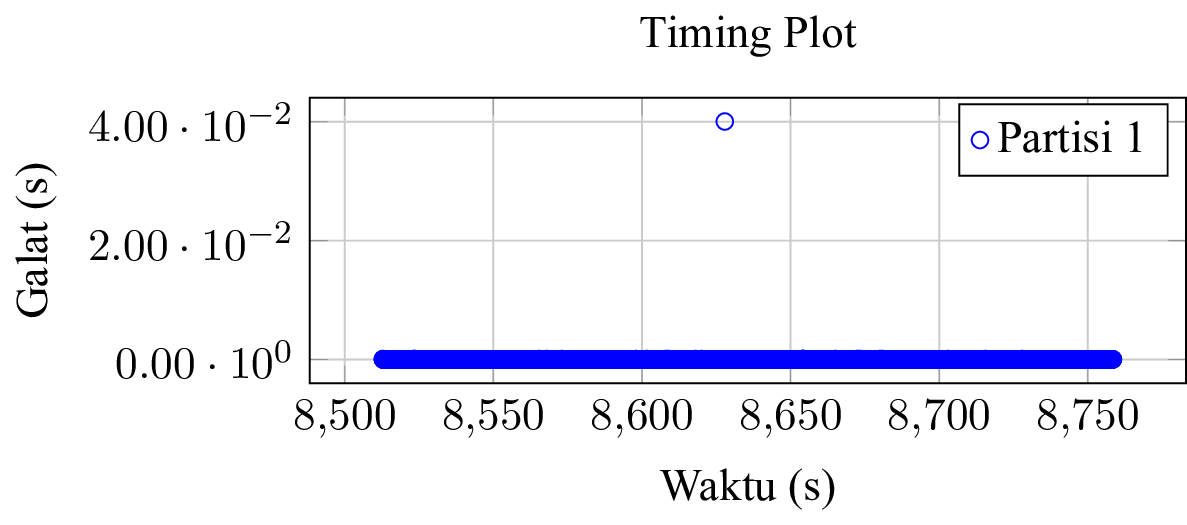
\includegraphics[scale=0.15]{latency-s2-error-p1.png}
			}
		\end{tabular}
		\caption{Hasil pengujian \textit{latency} skenario 2}
	\end{figure}

\end{frame}

\begin{frame}{Pengujian -- Pengujian \textit{Latency} (Skenario 3)}
	\begin{itemize}
		\item Jumlah layanan = 9 @ \SI{20}{\milli\second}.
		\item \textit{Major time frame} = \SI{180}{\milli\second}.
	\end{itemize}
\end{frame}
\begin{frame}{Pengujian -- Pengujian \textit{Latency} (Skenario 3)}
	\begin{figure}[htbp]
		\centering
		\begin{tabular}{c}
			\subfloat{
				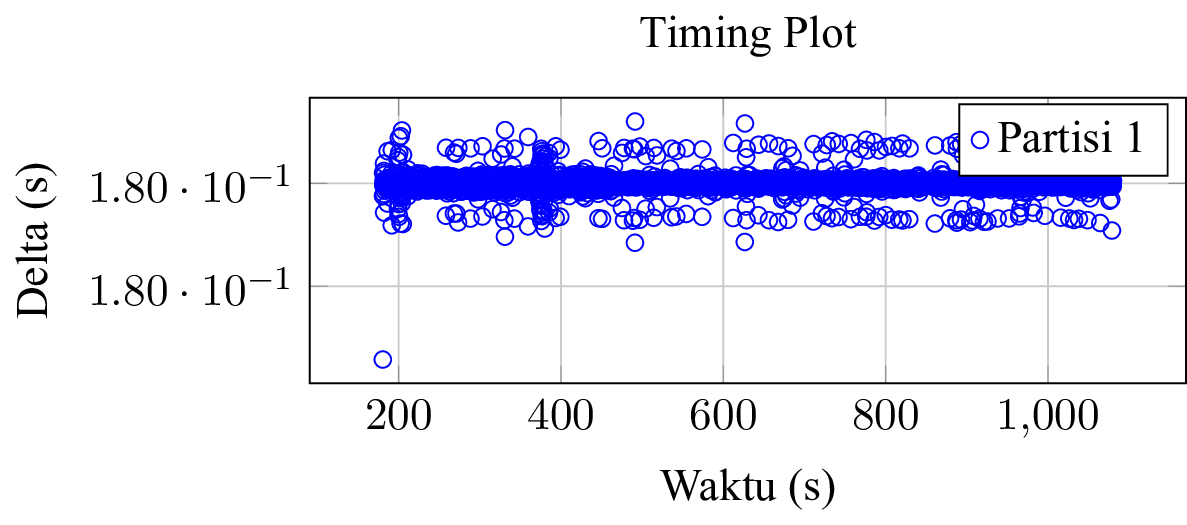
\includegraphics[scale=0.15]{./latency-s3-delta-p1.png}
			} \\
			\subfloat{
				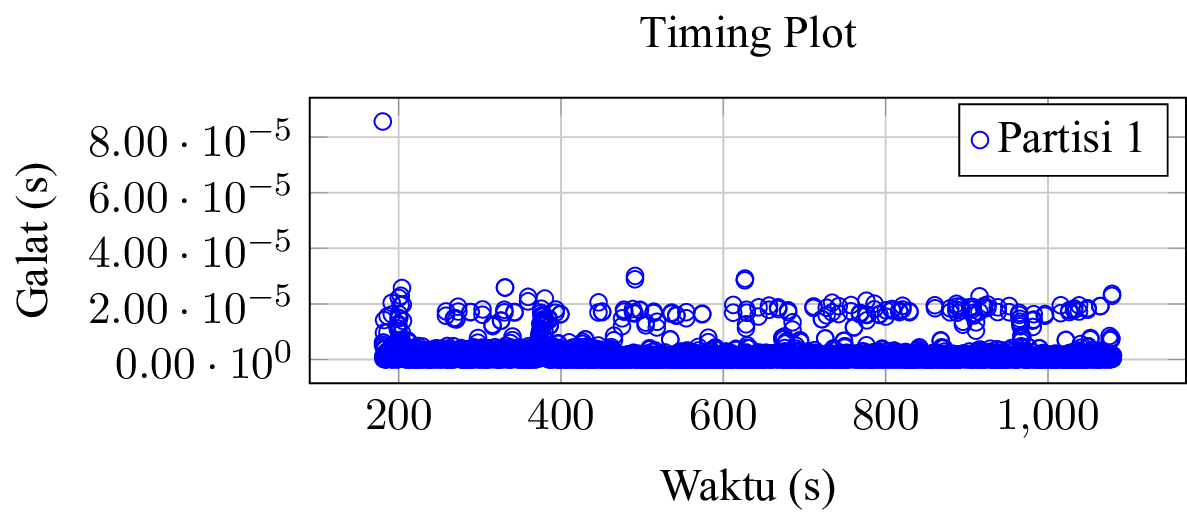
\includegraphics[scale=0.15]{./latency-s3-error-p1.png}
			}
		\end{tabular}
		\caption{Hasil pengujian \textit{latency} skenario 3 (hasil baik)}
	\end{figure}
\end{frame}

\begin{frame}{Pengujian -- Pengujian \textit{Latency} (Skenario 3)}
	\begin{figure}[htbp]
		\centering
		\begin{tabular}{c}
			\subfloat{
				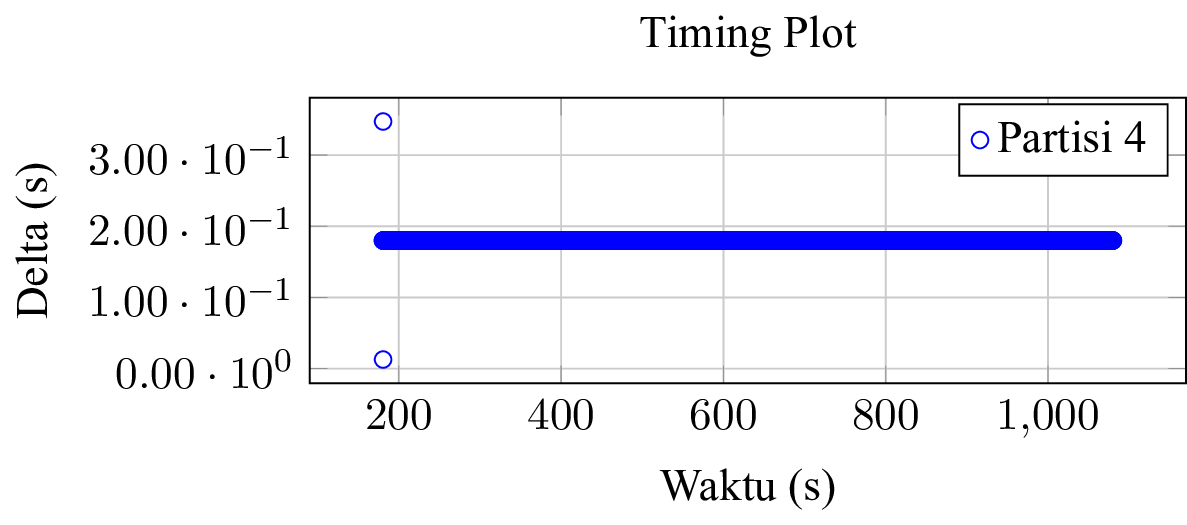
\includegraphics[scale=0.15]{./latency-s3-delta-p4.png}
			} \\
			\subfloat{
				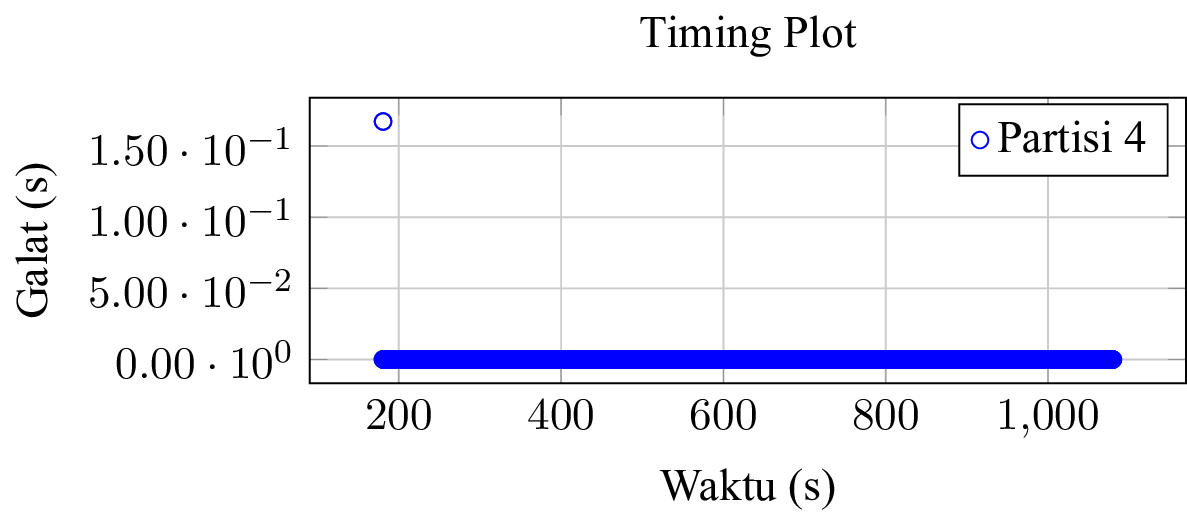
\includegraphics[scale=0.15]{./latency-s3-error-p4.png}
			}
		\end{tabular}
		\caption{Hasil pengujian \textit{latency} skenario 3 (hasil buruk)}
	\end{figure}
\end{frame}

\begin{frame}{Pengujian -- Kesimpulan Pengujian \textit{Latency}}
	\begin{enumerate}

		\item \textit{Periodic} task memiliki \textit{timing} yang
			sangat akurat apabila tidak ada partisi lain.

		\item \textit{Periodic} task memiliki \textit{timing} yang
			sangat jauh dari ekspektasi apabila terdapat beberapa
			layanan.

	\end{enumerate}
\end{frame}

\begin{frame}{Pengujian -- \textit{Time-drift}}
	\begin{itemize}

		\item Hasil pengujian sebelumnya menghasilkan pengukuran
			\textit{timing} yang buruk.

		\item Satu partisi vs Lebih dari satu partisi.

		\item Cek apakah waktu \textit{periodic task} berjalan dengan
			seharusnya.

		\item Time-drift \textit{task}

			\begin{equation}
				drift = now - (start + samples * expected)
			\end{equation}

	\end{itemize}
\end{frame}

\begin{frame}{Pengujian -- \textit{Time-drift}}
	\begin{figure}[htbp]
		\centering
		\begin{tabular}{c}
			\subfloat{
				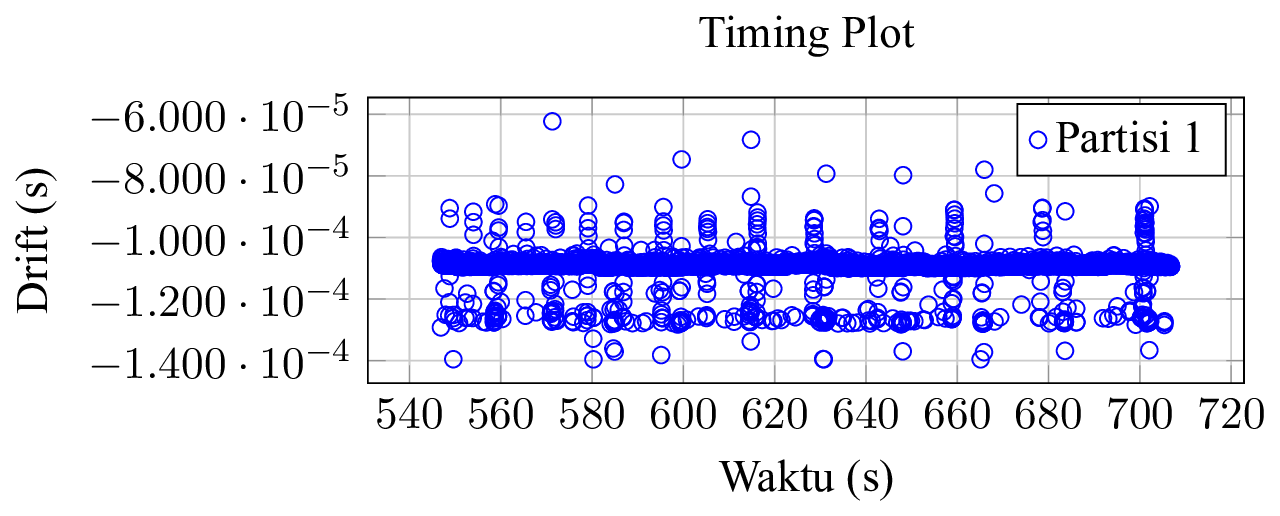
\includegraphics[scale=0.12]{./timedrift-s1.png}
			} \\
			\subfloat{
				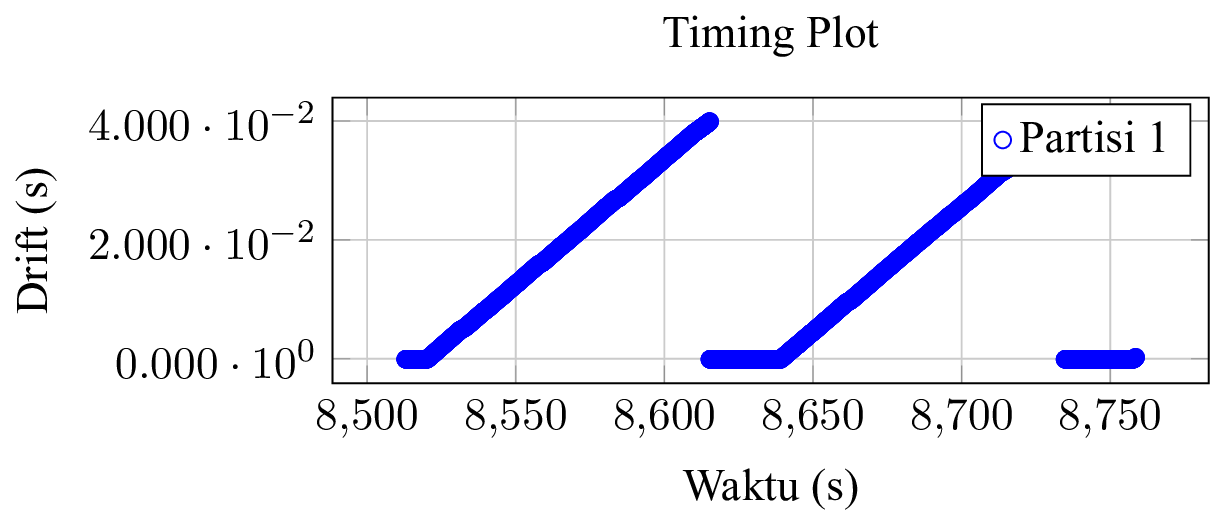
\includegraphics[scale=0.12]{./timedrift-s2-p1.png}
			}
		\end{tabular}
		\caption{Hasil pengujian \textit{time-drift}. Atas: Hasil pada sistem dengan satu layanan. Bawah: Hasil pada sistem dengan lebih daru satu layanan.}
	\end{figure}
\end{frame}

\section{Kesimpulan dan Saran}

\begin{frame}{Kesimpulan}
	\begin{itemize}
		\item \textit{Primary-backup partition scheduler} sudah diimplementasikan.
		\item \textit{Primary-backup partition scheduler} dapat menangani \textit{fault} pada partisi \textit{primary}.
		\item \textit{Primary-backup partition scheduler} dapat menangani \textit{fault} pada partisi \textit{backup}.
		\item Pengiriman informasi partisi sudah dapat dilakukan dengan menggunakan \textit{hypercall}.
		\item Sistem memiliki \textit{latency} yang buruk apabila terdapat pergantian partisi.
	\end{itemize}
\end{frame}

\begin{frame}{Saran}
	\begin{itemize}
		\item Perbaikan

			\begin{enumerate}
				\item \textit{Time-drift} pada sistem
				\item Kerangka pengujian
			\end{enumerate}

		\item Pengembangan

			\begin{enumerate}
				\item Minimalisasi penggunaan memori
				\item Pendeteksian kegagalan otomatis
				\item \textit{Multicore}
			\end{enumerate}
	
	\end{itemize}

\end{frame}

\begin{frame}[standout]
	\centering Demo
\end{frame}

\begin{frame}[standout]
	\centering Terima Kasih
\end{frame}

\section{Tambahan}
\begin{frame}
	\frametitle{Terminologi}
	\begin{itemize}
		\item \textit{Hypervisor} --- \textit{Supervisor} dari \textit{supervisor} (kernel), \textit{hyper} $>$ \textit{super}
		\item \textit{Open Source} --- Berlaku untuk perangkat lunak. Perangkat lunak tersedia bersama dengan \textit{source code}-nya.
		\item \textit{Time-Drift} --- Pergeseran waktu sistem karena ketidaktelitian perhitungan waktu atau perangkat sistem.
	\end{itemize}
\end{frame}

\end{document}
